% Standalone manuscript. Compile twice with xelatex -no-shell-escape.
% The chess mark uses DejaVu Sans; no external figure or bibliography file is required.
\documentclass[11pt,letterpaper]{article}
\usepackage{fontspec}
\setmainfont{Noto Serif}
\setsansfont{Noto Sans}
\setmonofont[Scale=.84]{DejaVu Sans Mono}
\newfontfamily\chessfont{DejaVu Sans}
\usepackage[margin=.94in,headheight=15pt]{geometry}
\usepackage{amsmath,amssymb,amsthm,mathtools}
\usepackage{microtype,booktabs,tabularx,longtable,array}
\usepackage{enumitem,algorithm,algpseudocode,placeins}
\algrenewcommand\textproc{\textsf}
\usepackage{tikz,xcolor,fancyhdr,titlesec,needspace,listings,etoolbox}
\usetikzlibrary{arrows.meta,positioning,calc,fit}
\usepackage[round,authoryear]{natbib}
\usepackage{xurl,hyperref}
\definecolor{ink}{HTML}{32224E}
\definecolor{muted}{HTML}{655D70}
\definecolor{wash}{HTML}{F4F1F8}
\definecolor{accent}{HTML}{65449A}
\hypersetup{colorlinks=true,linkcolor=ink,citecolor=ink,urlcolor=accent,
 pdftitle={Out-Strategise ♟: Transformational Intelligence for Constructing the Conditions of Success},
 pdfauthor={Vincent Boucher},
 pdfsubject={Joint observation and construction; exact strategic frontiers; purpose-specific inheritance; SUCCESSOR Omega},
 pdfkeywords={transformational intelligence, strategy synthesis, active diagnosis, robust planning, decision regions, SUCCESSOR Omega}}
\urlstyle{same}
\pagestyle{fancy}\fancyhf{}
\fancyhead[L]{\small\sffamily OUT-STRATEGISE}\fancyhead[R]{\small Boucher}
\fancyfoot[C]{\small\thepage}\renewcommand{\headrulewidth}{.35pt}
\setlength{\parindent}{1.1em}\setlength{\parskip}{.13em}
\setlength{\emergencystretch}{2em}\setlength{\tabcolsep}{5pt}\renewcommand{\arraystretch}{1.13}
\titleformat{\section}{\large\bfseries\color{ink}}{\thesection}{.65em}{}
\titleformat{\subsection}{\normalsize\bfseries}{\thesubsection}{.65em}{}
\titlespacing*{\section}{0pt}{1.1em}{.5em}\titlespacing*{\subsection}{0pt}{.75em}{.25em}
\setlist{nosep,leftmargin=1.5em,topsep=.2em}
\renewcommand{\topfraction}{.95}\renewcommand{\bottomfraction}{.85}
\renewcommand{\textfraction}{.06}\renewcommand{\floatpagefraction}{.85}
\newcolumntype{Y}{>{\raggedright\arraybackslash}X}
\newcolumntype{P}[1]{>{\raggedright\arraybackslash}p{#1}}
\newcommand{\Hset}{\mathcal H}\newcommand{\Pset}{\mathcal P}\newcommand{\Tset}{\mathcal T}
\newcommand{\Req}{\mathcal R}\newcommand{\K}{\mathcal K}
\newcommand{\Om}{SUCCESSOR~$\Omega$}
\newcommand{\insight}[1]{\begin{center}\setlength{\fboxsep}{9pt}\fcolorbox{ink}{wash}{\begin{minipage}{.92\linewidth}#1\end{minipage}}\end{center}}
\newtheorem{definition}{Definition}[section]
\newtheorem{proposition}{Proposition}[section]
\newtheorem{theorem}{Theorem}[section]
\newtheorem{corollary}{Corollary}[section]
\theoremstyle{remark}\newtheorem{remark}{Remark}[section]
\BeforeBeginEnvironment{theorem}{\Needspace{9\baselineskip}}
\BeforeBeginEnvironment{proposition}{\Needspace{8\baselineskip}}
\BeforeBeginEnvironment{definition}{\Needspace{7\baselineskip}}
\lstset{basicstyle=\small\ttfamily,breaklines=true,columns=fullflexible,keepspaces=true,
 showstringspaces=false,frame=single,rulecolor=\color{muted},aboveskip=.6em,belowskip=.6em}
\begin{document}
\thispagestyle{plain}
\begin{center}
{\small\sffamily\color{accent} MONTREAL.AI\quad /\quad TRANSFORMATIONAL INTELLIGENCE $\infty$\par}
\vspace{.75em}
{\fontsize{38}{42}\selectfont\bfseries\color{ink} Out-Strategise\hspace{.18em}{\chessfont ♟}\par}
\vspace{.6em}
{\Large\bfseries Transformational Intelligence for Constructing\par}
\vspace{.1em}
{\Large\bfseries the Conditions of Success\par}
\vspace{.85em}
{\large Vincent Boucher\par}
{MONTREAL.AI\par}
{Montréal, Québec, Canada\par}
\vspace{.5em}
{20 October 2026\quad$\cdot$\quad Research manuscript\par}
\end{center}
\begin{abstract}
A system can spend its intelligence discovering which action to take while accepting an unnecessarily restrictive set of actions. We study a different strategic object: a conditional construction that succeeds across possibilities the system still cannot distinguish. The technical question is not only what to learn, but what to build so that less must be learned. We develop an exact finite compiler that couples observation selection to a synthesized common completion, with a normal-form result specifying when construction may be deferred until commitment. For a grouped uncertain network we derive the complete minimax cost frontier under explicit assumptions and an exact purpose-specific quotient of its belief space. In a sixteen-world instance, a coarse observation followed by a constructed bypass costs seven units, versus eleven for the optimal observation-and-repair policy and twenty for the best construction without observation. The successful policy retains four possible faults: uncertainty remains, but no longer prevents the required delivery. The same family yields a checked 1,024-world policy of cost seven, against sixty-seven and 160 for those restricted alternatives. These are abstract operational costs, not model speedups. The quotient replaces 65,535 beliefs by 69 states in the anchor case, and agrees with an unquotiented reference on 75,967 belief cases across the study. A stricter successor purpose invalidates the old route and its abstraction; retained uncertainty supports a new four-unit extension instead of a false claim of inherited success. Thirty-two further directed acyclic graph instances are checked against independent module-subset enumeration. The contribution is a constructive, purpose-grounded account of when information, intervention, and representation should change together. It builds on decision-theoretic troubleshooting and robust planning; it does not demonstrate autonomous invention, physical deployment, or superiority to AlphaEvolve. The enduring asset is a method for constructing strategies that make available intelligence more effective without making the purpose easier.
\end{abstract}
\noindent\textbf{Keywords:} transformational intelligence; strategy synthesis; observation and construction; robust completion; capability inheritance; SUCCESSOR $\Omega$.
\begin{center}\small
\textbf{Find your Alpha. Build your SUCCESSOR $\Omega$.}\par
\href{https://github.com/MontrealAI/AGI-Alpha-Agent-v0}{github.com/MontrealAI/AGI-Alpha-Agent-v0}
\end{center}
\clearpage

\section{Do not only discover the winning move. Construct one.}
A delivery network has sixteen links, arranged in four consecutive groups. Exactly one original link has failed. An investigator can identify its group, inspect individual links, repair a particular link, or construct a reliable bypass around a group. The obligation is to deliver from the source to the destination. It is not to name the failed link.

One strategy diagnoses the failure precisely and repairs it. Another constructs enough redundancy to ignore all uncertainty. A third does something neither achieves efficiently: locate only the relevant group, then build a route that works regardless of which link inside it failed. The diagnosis is deliberately incomplete. The delivery is not.

The third strategy is not a more confident guess. It changes the available completion. It asks less of the investigator because it has constructed more of the world in which the investigator acts.

\insight{\textbf{Do not only discover which world you are in. Construct a move that succeeds in the worlds you cannot distinguish.}\par\smallskip The purpose stays fixed. The conditions for achieving it become an object of invention.}

This is the central move of \emph{Out-Strategise}. More capable models, more computation, and better coordination can improve a search. But they can also be spent resolving distinctions that a different construction would make irrelevant. Conversely, a little strategically chosen information can avoid an expensive universal construction. The object to optimize is the combination, not information or intervention in isolation.

\subsection{What changes relative to the preceding work}
\emph{Transformational Intelligence} makes the problem-solving formulation editable while keeping the authorized purpose as the reference \citep{boucherTI}. \emph{Invent the Economy} applies that idea to the joint construction of a capability and a feasible commercial arrangement \citep{boucherEconomy}. The three \emph{Capability Genesis} manuscripts preserve, identify, or construct scientific response interfaces under different assumptions \citep{packet}. \emph{Construct the Missing Experiment} then compiles an unresolved decision into additional experimental access and a measurement program \citep{boucherExperiment}.

The present paper challenges a remaining restriction: \emph{that an unresolved decision should primarily be repaired by acquiring information for a fixed set of acceptable actions}. Sometimes the decisive construction is not a better observation. It is a new executable completion whose success region covers several still-possible worlds. The earlier observation constructor remains a useful component, but it is no longer the only way to remove an obstruction.

Boden's distinction between exploring and transforming conceptual spaces supplies an earlier intellectual context \citep{boden}. This is not a claim that robust action, repair, or learning before acting are new. Decision-theoretic troubleshooting already combines observations, repairs, and reconfiguration; planning under partial observability and uncertain routing with neutralization supply close precedents \citep{breese,kaelbling,traveler}. Our scoped contribution is an executed joint-construction compiler, an analytic frontier and exact quotient for a particular family, and a successor counterexample showing why strategic sufficiency must be indexed by purpose. The claims should be judged at that strength.

\subsection{The central result in one table}
The reference costs are supplied abstract units: a group alarm costs 2; inspecting a link costs 2; repairing it costs 3; constructing a group bypass costs 5. They are not dollar estimates or physical quotations.

\begin{table}[htbp]\centering\small
\caption{Exact worst-case costs in the sixteen-world model. Each successful strategy serves the same source-to-destination obligation. The last row changes the construction vocabulary, not the required outcome.}\label{tab:hero}
\begin{tabularx}{\linewidth}{@{}YP{.36\linewidth}r@{}}\toprule
Strategy class & What must be resolved & Cost\\\midrule
Best construction without observations & Nothing; protect every group & 20\\
Best observations plus individual repairs & Enough to choose repairs economically & 11\\
Require exact fault identity, with all modules available & One precise fault & 11\\
Joint observation and constructed completion & The failed group, not its internal fault & \textbf{7}\\\bottomrule
\end{tabularx}
\end{table}

The reference compiler emits the actual conditional plan and its route. A separate checker verifies every branch against every compatible world. The lower cost does not establish a smarter model: no language model runs inside the experiment. It establishes the consequence of changing what the strategy is allowed to construct.

\section{A strategy can remove the need to know}
\label{sec:semantics}
\subsection{Preserve the purpose; change the completion}
Let $q$ denote an authorized purpose with material outcome requirements, permitted actions, and a declared resource account. Let $\Hset$ be a finite set of possible fixed worlds, and let $B\subseteq\Hset$ be the nonempty set compatible with the retained observations. The model class is supplied, not inferred to be complete from a successful run.

A completion program $p$ is an executable composition of available operations and constructible modules. Its success region is
\begin{equation}
\Req_q(p)=\{h\in\Hset:p\text{ satisfies the unchanged purpose }q\text{ in }h\}.
\end{equation}
The program can change the effective system: add a reliable route, replace a component, or install a separately admitted capability. It must account for its construction costs and side effects. An action is robustly sufficient at $B$ exactly when $B\subseteq\Req_q(p)$.

\begin{definition}[Construction envelope]
For installed assets $I$ and an admitted program language $\Pset_I$, define
\begin{equation}\label{eq:envelope}
K_{q,I}(B)=\min_{p\in\Pset_I:\ B\subseteq\Req_q(p)} C_I(p),
\end{equation}
with $K_{q,I}(B)=\infty$ if no common completion exists. $C_I(p)$ is the incremental operational cost under the declared accounting; assets already in $I$ are not purchased twice.
\end{definition}
The envelope is an optimization problem, not a presumed oracle. Section~\ref{sec:compiler} gives an executable construction for directed acyclic graphs and a separate exhaustive checker. Changing the program language changes the envelope. The model therefore admits a practical distinction between selecting an existing action and constructing a new composite completion from permitted parts.

\subsection{A common completion is stronger than a world-by-world possibility}
The following quantifiers are not interchangeable:
\begin{equation}\label{eq:quantifiers}
\underbrace{\forall h\in B\ \exists p:\ h\in\Req_q(p)}_{\text{each world is individually solvable}}
\qquad\not\Rightarrow\qquad
\underbrace{\exists p\ \forall h\in B:\ h\in\Req_q(p)}_{\text{one executable choice works without knowing }h}.
\end{equation}
A two-branch diamond exposes the difference. In one world the left branch is blocked; in the other the right branch is blocked. Each world has a route, but no fixed route works in both. With no informative test and no permitted modification, robust completion is impossible. The reference executes this control. Taking the union of possible edges and finding a path would give a fictitious solution.

For the stated single-commitment contract, the right object is a path in the graph of \emph{jointly usable} edges. If the execution itself may inspect and switch branches, that adaptive behavior must be part of $p$ and its cost. It cannot be silently imported into a proof about a fixed final path.

\subsection{Separate the worlds or make their difference immaterial}
Relative to a fixed completion language, call $W\subseteq B$ an obstruction when no program in that language succeeds throughout $W$. If a policy receives identical observations in every world in $W$, it chooses the same final program there. Consequently, a guaranteed policy must either obtain a distinction that splits $W$, or construct a completion whose success region includes the still-common worlds.

This elementary \emph{separate-or-neutralize} principle is a useful design obligation, not a new impossibility theorem for general intelligence. It tells a constructor what a failure witness means. A missing observation is one response. A new common action is another. The latter does not make the worlds identical, remove the fault, or update the belief to a more convenient singleton. It makes the difference irrelevant to the specified outcome.

Decision-region methods already avoid demanding complete identification when a common decision is sufficient \citep{javdani}. Here the region can be produced by an explicitly costed construction rather than supplied solely as a fixed action label. The compiler must return that construction, not merely claim that some robust option ought to exist.

\section{An exact compiler for learning and building}
\label{sec:compiler}
\subsection{The diagnose--prepare--commit boundary}
The reference model uses deterministic, nondestructive tests $t:\Hset\to Y_t$ with positive costs $c_t$. A test reads the unchanged original system. Construction modules may be prepared, but are activated only for the final completion. Their prices, availability, permissions, and success conditions do not depend on the timing of earlier preparations. There are no intervening delivery deadlines, safety rewards, or observations caused by preparation itself.

These assumptions are substantive. They apply to a bounded planning problem in which diagnosis and preparation precede one commitment. They do not describe arbitrary troubleshooting in a changing plant. A repair that changes subsequent sensor readings, or a fixture needed to obtain a reading at all, requires an expanded state including the current construction.

\begin{proposition}[Deferred-construction normal form]\label{prop:postpone}
Under the boundary above, nonnegative construction costs, and no benefit from a prepared module before final commitment, every feasible policy has a policy of no greater worst-case cost in which all construction occurs after the last informative test. The final construction may depend on the observed branch.
\end{proposition}
\begin{proof}
Keep the original test sequence on each observation branch. Preparation changes neither the test result nor its availability, so the branch remains well defined. At a terminal node, prepare and activate the modules used by that branch's final completion, omitting earlier purchases that are no longer needed. This produces the same valid completion at no greater module cost. Test costs are unchanged. The transformation holds on each world and hence for their worst case.
\end{proof}

The proposition is a model reduction, not a command to postpone every real investment. It fails when installation opens a test, prices change, early service matters, or observations depend on the modified plant. The point is to derive when a smaller state is legitimate rather than assume that all strategic history can be discarded.

\subsection{Joint optimality with a constructed terminal action}
For a test $t$, let $\mathcal P_t(B)$ be its partition into nonempty compatible cells. Noninformative tests have one cell equal to $B$ and are omitted. The exact worst-case operational value is
\begin{equation}\label{eq:bellman}
\boxed{\quad V_{q,I}(B)=\min\left\{K_{q,I}(B),\ \min_{t:\,|\mathcal P_t(B)|>1}
\left[c_t+\max_{B'\in\mathcal P_t(B)}V_{q,I}(B')\right]\right\}.\quad}
\end{equation}
The inner minimum is $\infty$ when no informative test exists. Every child is a proper subset, so the recurrence is acyclic. An infinite value means no guaranteed completion within the supplied language and tests.

\begin{theorem}[Exact finite synthesis]\label{thm:dp}
If the construction envelope and test partitions are evaluated exactly, Equation~\eqref{eq:bellman} returns the minimum worst-case cost over all finite deterministic policies admitted by the diagnose--prepare--commit model. Backtracking its minimizers returns a feasible policy attaining every finite value.
\end{theorem}
\begin{proof}
Induct on $|B|$. A policy either commits immediately, at cost at least $K(B)$, or performs an informative first test. An uninformative test only incurs positive cost and can be removed. For an informative test, each child has smaller cardinality and its best continuation has the inductively established value. The worst branch therefore costs at least the corresponding term in Equation~\eqref{eq:bellman}. Choosing a minimizing term and its attaining continuations realizes the bound. Singleton beliefs give the base case. Proposition~\ref{prop:postpone} covers permitted interleavings of preparation and tests.
\end{proof}

This specializes Bellman optimality by adding a construction subproblem; it does not introduce a new dynamic-programming principle \citep{kaelbling}. Its significance is the complete object returned: the observation program, the branch-specific construction, the unchanged outcome check, and the uncertainty that remains.

\subsection{How the envelope is actually computed}
The reference accepts a forward directed acyclic graph. A base edge may be unusable in some supplied worlds. Each optional module adds one named edge with a nonnegative integer installation cost. Previously installed modules cost zero incrementally. A purpose requires a source-to-destination path visiting an ordered list of mandatory checkpoints.

For belief $B$, delete every edge failing in at least one $h\in B$. Keep reliable optional edges with their incremental construction weights. A shortest path through the required checkpoints minimizes $K(B)$ and returns its explicit module composition. The graph is acyclic and each module adds one edge, so a route never pays twice for the same module. Between ordered checkpoints, ordinary forward dynamic programming suffices. General modules that add multiple edges, interfere, or require shared setup need a different construction solver.

The observation planner memoizes Equation~\eqref{eq:bellman}. In the general case it can still visit exponentially many beliefs. The implementation is an exact research compiler for small explicit models, not a scalable solution to arbitrary partially observable planning. Its output has a finite JSON representation with the exact residual world indices at every node, observation labels, a common route at each leaf, computed cost, and a model digest. The record explicitly grants no operating authority.

\begin{algorithm}[htbp]\small
\caption{Out-Strategise: exact reference construction}\label{alg:main}
\begin{algorithmic}[1]
\Require Purpose and checkpoints; worlds; tests; constructible modules; costs; installed assets
\Function{Solve}{$B$}
  \State Reject an empty or inconsistent belief
  \State Construct the least-cost route valid throughout $B$; retain its modules
  \For{each test that splits $B$}
    \State Solve its nonempty residual cells recursively
    \State Compare test cost plus worst continuation with the common route's cost
  \EndFor
  \State Retain the least-cost executable alternative and all unresolved worlds
  \State \Return its value and conditional construction record
\EndFunction
\State Check every observation branch and every leaf route separately
\State Recompile if purpose, model, costs, module semantics, or permissions change
\end{algorithmic}
\end{algorithm}

\section{A complete strategic frontier for grouped uncertainty}
\label{sec:frontier}
The chain family makes the interplay among information and construction analytically legible. It also gives an exact large-instance result without pretending that an exponential generic solver has become universally fast.

There are $m$ consecutive groups of $k$ original links. Exactly one of the $mk$ links has failed. A coarse alarm returns its group at cost $c>0$. A fine inspection names whether a particular original link failed, at cost $t>0$. A reliable parallel repair of any one link costs $r>0$. A reliable bypass around an entire group costs $b\ge0$. The obligation is passage through the chain to its destination; there is initially no requirement to visit every internal link. All options and their semantics are available to every unrestricted comparator.

\Needspace{12\baselineskip}
\subsection{First decide what one unresolved group is worth}
\begin{theorem}[One-group frontier]\label{thm:one}
If one group contains $k\ge1$ still-possible fault locations, the exact minimum worst-case cost is
\begin{equation}\label{eq:one}
v(k)=\min\{b,\ kr,\ r+(k-1)t\}.
\end{equation}
The three terms are bypass the group, repair every possible link, and inspect until the failed link is known and repair it. For a repair-only vocabulary, omit the bypass term.
\end{theorem}
\begin{proof}
An inspection that finds the failed link ends the information problem. The adversarial branch instead reports healthy links until the remaining set is small enough to commit. After $j$ such observations, $0\le j\le k-1$, a robust completion costs $\min\{b,(k-j)r\}$. Earlier positive branches cost no more than the corresponding worst negative branch. Thus the optimum is
$\min_{0\le j<k}[jt+\min\{b,(k-j)r\}]$.
The bypass branch is minimized at $j=0$. The repair branch is $kr+j(t-r)$, minimized at one of the two endpoints. This yields Equation~\eqref{eq:one}. No other informative test is present within a known group.
\end{proof}

The optimum does not insist on localization. If replacement is cheaper than diagnosis, repairing all remaining candidates is valid. If a bypass is cheaper still, the fault need not be identified at all. A repair-only baseline is therefore allowed to make the best such tradeoff; it is not forced to waste tests.

\subsection{Coarse information and robust construction can be complementary}
\begin{theorem}[Grouped root frontier]\label{thm:root}
For $m\ge2$, equal group size $k$, the model above, and $c\le t$, the exact root value is
\begin{equation}\label{eq:root}
\boxed{V(m,k)=\min\left\{m\min(b,kr),\ c+\min\bigl(b,kr,r+(k-1)t\bigr)\right\}.}
\end{equation}
\end{theorem}
\begin{proof}
With no observation, a common route must protect each group against every possible internal fault. Its cost is $m\min(b,kr)$. A coarse alarm reduces the task to one unresolved group and attains $c+v(k)$. If a fine inspection is performed first, an adversary may place the fault in another group, leaving an entire untested group of size $k$. Even granting its identity for free, the remaining cost is at least $v(k)$. That first inspection therefore costs at least $t+v(k)\ge c+v(k)$. These exhaust the possible first decisions under the normal form.
\end{proof}

This is a complete conditional frontier, not merely a favored example. It identifies the region where partial information followed by a robust construction strictly beats both observation-free construction and the best repair-only strategy. When $c>t$, the lower-bound argument no longer selects the coarse alarm. The general recurrence remains valid and the executed grid contains cases where a fine inspection should come first.

A particularly transparent regime is
\begin{equation}\label{eq:region}
b<\min\{kr,r+(k-1)t\},\qquad c<(m-1)b.
\end{equation}
Then $V(m,k)=c+b$: locate the group and bypass it. The group alarm alone leaves an expensive internal diagnosis; the bypass vocabulary alone leaves an expensive universal construction. Together they change which distinctions must be resolved.

\begin{figure}[htbp]\centering
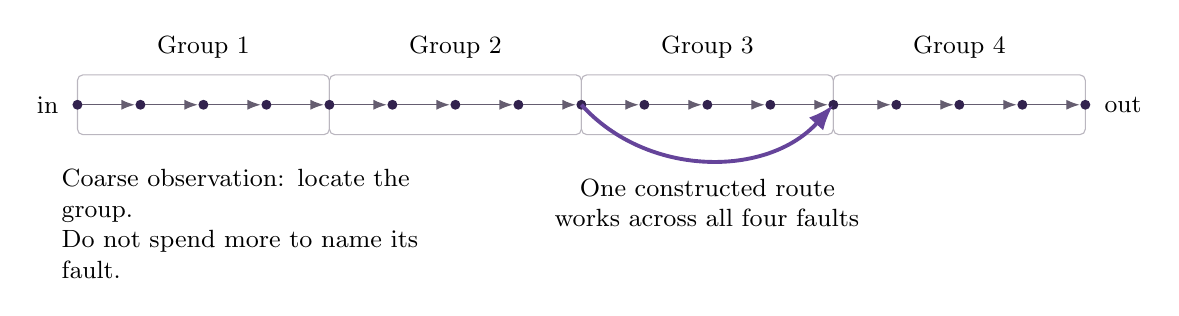
\begin{tikzpicture}[>=Latex,font=\small,x=.8cm,y=1cm]
\foreach \g in {0,1,2,3}{
 \pgfmathsetmacro{\left}{4*\g}
 \pgfmathsetmacro{\right}{4*\g+4}
 \draw[draw=muted!45,rounded corners=2pt] (\left,-.38) rectangle (\right,.38);
 \node[above] at ({\left+2},.46) {Group \the\numexpr\g+1\relax};
}
\foreach \i in {0,...,16}{\fill[ink] (\i,0) circle (1.8pt);}
\foreach \i in {0,...,15}{\draw[->,draw=muted] (\i+.08,0)--(\i+.91,0);}
\draw[->,line width=1.4pt,draw=accent] (8,0) to[bend right=48] node[below=3pt,align=center,text width=5.7cm]{One constructed route\\works across all four faults} (12,0);
\node[below,align=left,text width=5.2cm] at (3,-.7) {Coarse observation: locate the group.\\Do not spend more to name its fault.};
\node[left] at (-.15,0) {in};\node[right] at (16.15,0) {out};
\end{tikzpicture}
\caption{The hero policy after the alarm identifies the third group. A reliable bypass is a supplied constructible primitive; the compiler selects and composes it into a route valid in all four remaining worlds. Internal links are means, not mandatory processing steps. Later checkpoint requirements can invalidate this route.}\label{fig:hero}
\end{figure}

\subsection{A conditional separation that grows with the inherited restriction}
With $c=t=2$, $r=3$, $b=5$, and $m,k\ge2$, the joint value is seven. Observation-free protection costs $5m$. The optimal repair-only value is $2k+3$; in this parameter regime identifying the last candidate by elimination is cheaper than repairing all of them.

Holding these supplied prices fixed, the two restricted costs grow with group count or width while the joint cost remains seven. This is an unbounded separation between named formulations in the mathematical family. It is \emph{not} a law that a physical bypass of arbitrary size always costs five units, an infinite intelligence multiplier, or evidence that a rival AI is incapable of choosing the same construction. In real networks, span, reliability, lead time, and capacity can make $b$ grow.

\subsection{Information is valuable relative to what can be built}
With a free reliable bypass, constructing around every group costs zero and no positive-cost observation is useful. With an expensive bypass, diagnosis and repair become preferable. Between those extremes, coarse information is worth buying because it selects where to build, while fine information is not worth buying because the construction absorbs its unresolved distinctions.

This supplies an operational answer to a recurring strategic mistake: estimating the value of information under an unnecessarily fixed action set. The price of learning and the price of making learning unnecessary have to be compared together. The result is not ``never diagnose'' or ``always build redundancy.'' It is the explicit frontier in Equation~\eqref{eq:root}.

\section{Make the planning problem smaller without making the purpose smaller}
\label{sec:quotient}
A good strategy can make a given solver more effective by changing the representation it must search. The chain family has exponentially many possible beliefs. Under its uniform costs and endpoint-only purpose, most labels do not matter to the optimal value.

For a belief $B$, let $n_g$ be the number of candidate failed links remaining in group $g$. Remove zero entries and sort the positive counts. Call the resulting tuple $s(B)$. Groups with identical candidate counts are interchangeable for this purpose, even though their physical locations remain necessary when emitting the route.

\begin{theorem}[Purpose-specific count quotient]\label{thm:quotient}
For the grouped model with uniform module and test costs, unchanged endpoint-only purpose, and any positive $c,t,r$ and nonnegative $b$, $V(B)$ depends only on $s(B)$. The quotient has
\begin{equation}\label{eq:states}
\binom{m+k}{k}-1
\end{equation}
possible nonempty count states, rather than $2^{mk}-1$ possible nonempty beliefs.
\end{theorem}
\begin{proof}
For state $(n_1,\ldots,n_\ell)$, the robust completion cost is $\sum_i\min(b,rn_i)$. A coarse alarm has children $(n_i)$. Inspecting a candidate in a group of size $n$ has a positive child $(1)$ and a negative child formed by replacing $n$ by $n-1$, deleting zero and sorting. The costs and quotient children are therefore determined entirely by the tuple. Induction on $\sum_i n_i$ in Equation~\eqref{eq:bellman} proves value equivalence and permits a concrete action to be lifted by choosing any matching group and candidate. The number of multisets of at most $m$ elements from $\{1,\ldots,k\}$ is $\binom{m+k}{k}$, including the empty multiset; subtract one.
\end{proof}

This is an exact specialization of established value-preserving model reduction, not the first use of bisimulation or aggregation in planning \citep{givan}. Its practical importance here is that the constructed representation is paired with the real outcome semantics. For four groups of four links, 65,535 beliefs reduce to 69 count states. For sixteen groups of four, the corresponding counts are $2^{64}-1$ and 4,844.

The reduction is not polynomial in both $m$ and $k$. For 32 groups of 32, even the count-state bound is enormous. The large reported instance uses the closed-form frontier and an emitted policy, not exhaustive quotient enumeration. The two mathematical constructions solve different costs: the quotient reduces a finite dynamic program; the frontier eliminates that program for its restricted symmetric root.

\subsection{Compression is not permission to forget the world}
The artifact retains the full residual belief and the mapping from groups to original links. The count tuple is an internal planning representation, not a sufficient replacement for all future knowledge. A new purpose can make group location or link position decisive. An inherited strategy must then re-establish the abstraction's validity rather than reuse it because it was once optimal.

This carries a central lesson of the predecessor manuscripts into strategy itself: an apparently irrelevant distinction can matter after an intervention or a changed question \citep{packet}. What is safe to compress is relative to the full declared continuation, not only the first successful output.

\section{Executed results and independent implementation checks}
\label{sec:results}
\subsection{What was supplied and what the program constructed}
The model family, failure lists, primitive tests, costs, bypass and repair semantics, and goals are author supplied. The program computes the observation policy, route composition, remaining beliefs, exact costs, and the comparison records. It does not discover a physical bypass technology, infer the fault laws from unstructured data, or learn a new discovery policy.

The reference is standard-library Python using integer costs. The forward shortest-path constructor is checked by a separately implemented solver that enumerates module subsets and verifies common reachability. The conditional policy checker independently recomputes observation branches, verifies the same route in every compatible world, enforces all checkpoints, and sums actual module costs. A certificate proves only those declared semantics. It does not prove model completeness or independent physical truth.

\subsection{The sixteen-world construction}
All sixteen world executions of the selected policy cost seven. Each branch uses one coarse observation and one group bypass. Each leaf retains four worlds. The best repair-only policy costs eleven; requiring precise identity even with bypasses available also costs eleven. Removing the coarse alarm raises the best joint policy's cost to twenty in this instance.

The unrestricted raw-belief solver evaluates all 65,535 nonempty subsets and agrees with the count quotient on every value. This is an exhaustive software comparison for the fixture, not 65,535 independent examples of invented strategies. All computations share the supplied semantics and authorship.

\begin{table}[htbp]\centering\small
\caption{Scale within the proved grouped family, with $(c,t,r,b)=(2,2,3,5)$. Every emitted policy is checked against every listed world. These are alternative single-failure worlds, not independent simultaneous faults. Costs are operational units.}\label{tab:scale}
\begin{tabular}{@{}rrrrrr@{}}\toprule
Groups & Links/group & Worlds & Joint & Repair-only & No observation\\\midrule
2 & 2 & 4 & 7 & 7 & 10\\
4 & 4 & 16 & 7 & 11 & 20\\
8 & 8 & 64 & 7 & 19 & 40\\
16 & 4 & 64 & 7 & 11 & 80\\
16 & 16 & 256 & 7 & 35 & 80\\
32 & 32 & 1,024 & \textbf{7} & 67 & 160\\\bottomrule
\end{tabular}
\end{table}

The four-world tie matters. A transformation is not required to win in every instance. At high bypass cost, the compiler retains diagnosis and repair; at zero bypass cost, it commits without buying information. These controls test the selection rule rather than reward any construction merely for being called transformational.

\subsection{Parameter coverage and general graph checks}
A grid crosses $m,k\in\{2,3,4\}$, $c,t\in\{1,2,4\}$, $r\in\{1,3,5\}$, and $b\in\{2,5,9\}$, giving 729 cases. All 486 cases satisfying $c\le t$ match the closed-form root frontier. The exact count planner selects immediate construction in 111 cases, the coarse alarm in 610, and a fine inspection in eight. Joint synthesis is strictly cheaper than both restricted alternatives in 315 cases and ties the repair-only optimum in 342. These are counts in an author-selected grid, not estimates of market prevalence or real-world success rates.

A further 64 parameter cases with $m,k\in\{2,3\}$ are compared on every nonempty raw belief. Their 10,432 checks, added to the anchor's 65,535, give 75,967 raw-belief/quotient agreements.

To test the generic constructor outside the grouped topology, the driver generates 32 forward directed acyclic graphs with six vertices, five supplied worlds, six optional edge modules, and three supplied tests. Some worlds contain two failed base edges; the generic solver uses their actual failure lists rather than the grouped theorem. The complete cases and code digests are saved before evaluation. All 992 nonempty belief cases agree with the separate module-subset/reachability and raw-belief reference. Thirty root cases are feasible and two are not.

These are additional software-confirmation inputs, not externally blinded tasks or independent scientific replications. Changing from a chain to a general graph exercises a different combinatorial topology; it is not evidence of transfer to a physical industry.

\begin{table}[htbp]\centering\small
\caption{Evidence ledger. The counts concern exact synthetic computations, not model-generated discoveries.}\label{tab:coverage}
\begin{tabularx}{\linewidth}{@{}YrY@{}}\toprule
Check & Count & Meaning\\\midrule
Anchor world executions & 16 & Every emitted branch serves its modeled purpose\\
Largest policy's world checks & 1,024 & All modeled fault locations covered\\
Root parameter cases & 729 & Strategy regimes and decline cases\\
Closed-form root comparisons & 486 & Cases satisfying the theorem's premises\\
Raw-belief/quotient comparisons & 75,967 & Exact agreement without symmetry in the reference\\
Generic graph belief comparisons & 992 & 32 instances; exhaustive module-subset alternative\\
Unit-test methods & 41 & Functional, boundary, tampering, and source-binding checks\\\bottomrule
\end{tabularx}
\end{table}

\subsection{What ``fixed intelligence'' does not mean here}
The numerical construction makes no language-model, external-service, or wallet calls. It is AI-assisted authored research, not a controlled experiment in which a model discovers the transformation. Both unrestricted implementations receive the same permitted options and tie on the tested optima. No claim of defeating AlphaEvolve, an expert engineer, or another frontier agent follows.

The initial complete reference run took about 21.43 seconds in the recorded Python 3.13.5 environment. This includes generating results and exhaustive checks; it is not a benchmark of operational deployment or a timing comparison against another research system. Authoring, literature review, proof development, integration, physical validation, energy, and customer work are not measured by that timer. The reported seven units count only the supplied observation and construction operations.

The relevant contribution is a demonstrated formulation-dependent cost frontier and a smaller exact representation. A future model comparison must hold model access, initial assets, tools, permissions, and total campaign resources comparable, while allowing every competitor to construct the same kinds of alternatives.

\section{A stronger successor must sometimes reject its parent's winning move}
\label{sec:successor}
After the anchor alarm identifies group 3, the retained belief is $\{8,9,10,11\}$ in zero-based edge indexing. The installed bypass connects node 8 to node 12. The old route delivers to node 16, but does not locate the fault. This is a valid historical result.

Now change the authorized purpose: delivery must pass through node 10 before reaching node 16. Node 10 is a required checkpoint, not an optional implementation detail. The old bypass skips it. Importing the old approval cannot make that route satisfy the new obligation.

The new admitted construction menu adds a left-half bypass $8\to10$ and a right-half bypass $10\to12$, each costing three. A new half-alarm costs one and indicates which half contains the original fault. These primitives are supplied and separately authorized in the modeled successor; the compiler does not invent their physical feasibility.

The emitted extension reads the half-alarm, constructs only the affected half-bypass, and uses healthy original links on the other half. It costs four additional units and is checked in all four remaining worlds. Constructing both half-bypasses without the new reading costs six. Removing the new half-alarm from the available tests also makes the optimum six.

\begin{figure}[htbp]\centering
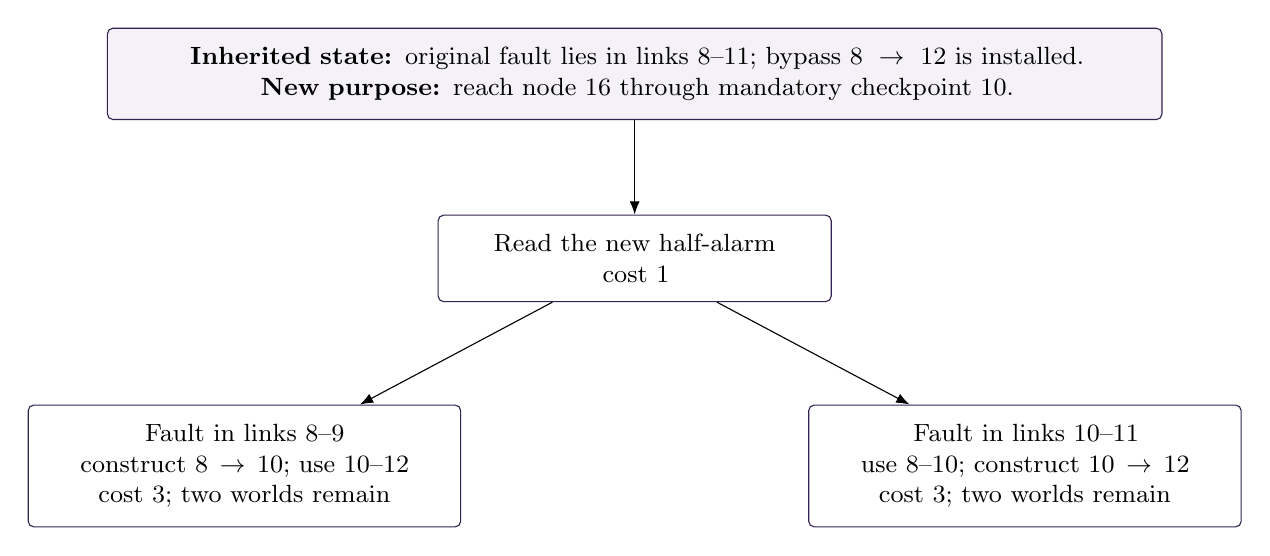
\begin{tikzpicture}[>=Latex,font=\small,node distance=12mm,
 box/.style={draw=ink,rounded corners=2pt,align=center,inner sep=7pt}]
\node[box,text width=12.9cm,fill=wash] (root) {\textbf{Inherited state:} original fault lies in links 8--11; bypass $8\to12$ is installed.\\
\textbf{New purpose:} reach node 16 through mandatory checkpoint 10.};
\node[box,below=of root,text width=4.5cm] (test) {Read the new half-alarm\\cost 1};
\node[box,below left=13mm and -3mm of test,text width=5.0cm] (left) {Fault in links 8--9\\construct $8\to10$; use 10--12\\cost 3; two worlds remain};
\node[box,below right=13mm and -3mm of test,text width=5.0cm] (right) {Fault in links 10--11\\use 8--10; construct $10\to12$\\cost 3; two worlds remain};
\draw[->] (root)--(test);\draw[->] (test)--(left);\draw[->] (test)--(right);
\node[below=10mm of test,opacity=0] {x};
\end{tikzpicture}
\caption{A successor inherits a valid model and remaining uncertainty, not an unconditional winning action. The old route is rejected. The new policy preserves the stronger checkpoint purpose without demanding exact fault identity. No hardware is installed by the reference program.}\label{fig:successor}
\end{figure}

\subsection{An optimal abstraction can become the wrong memory}
The count quotient is exact for the endpoint-only task. It is not exact for every future purpose. Consider a new destination at node 2. Beliefs $\{0,1\}$ and $\{2,3\}$ both have the old count summary $(2)$. Yet their common-completion costs are six and zero respectively: faults before the new destination require repair, while faults beyond it do not affect that delivery. The group bypass overshoots node 2 and cannot serve as an admissible route.

This exact counterexample explains why the portable record retains full residual worlds and task semantics. A purpose-specific quotient can accelerate current planning while leaving the evidence needed to build a different quotient later. Retaining only the quotient would lose information the successor needs.

\subsection{What was inherited, and what was paid again}
The successor reuses the identity of the still-compatible original faults, the unchanged original test semantics, the graph, and the historical asset record. It pays for the new observation and newly used modules. Its checker enforces the new checkpoint. The earlier bypass is not charged again, but its historical five-unit cost has not vanished from lifetime accounting.

The anchor-plus-extension path costs eleven units. This is not claimed to beat planning from the outset for the stronger final purpose. The point is purpose-sensitive continuation: the system knows when its former answer is inadequate and constructs the next admissible strategy from retained evidence. It does not claim a universally improving sequence of policies or automatically learn a better discovery procedure.

\section{Failure is part of the mechanism, not a footnote}
\label{sec:failure}
\subsection{A valid model certificate can fail in the world}
The anchor assumes exactly one original failure. Add an unmodeled failure at edge 0 while the modeled fault lies in group 3. The selected group-3 bypass does not protect edge 0, and the route fails. The checker rejects it when that extra failure is explicitly supplied. It cannot infer an undisclosed extra failure from a file digest or from arithmetic consistency.

A physical or software deployment must therefore justify failure coverage, test fidelity, module reliability, intervention side effects, and source identity. A broadened failure set can make a more expensive construction or further observation necessary. Repetition of the old diagnostic cannot compensate for a false model premise by declaration.

\subsection{When the normal form does not apply}
Suppose a one-unit inspection fixture must be installed before a sensor can distinguish two worlds. A planner that admits tests only on the original uninstrumented system cannot use that sensor. Conversely, pretending the sensor is free before construction understates the cost. The correct state includes which tests the installed fixture enables.

Similarly, a repair-and-observe action changes future observations and belongs to a dynamic troubleshooting model, not the static test partition used here. Deadlines, irreversible actions, stochastic damage, changing prices, or rewards for early partial service can also invalidate deferred construction. The normal form states a sufficient modeling boundary, not a general instruction to postpone investment. Existing troubleshooting and partially observable planning methods explicitly address richer interactions \citep{breese,kaelbling}.

\subsection{When the transformation should lose}
An expensive bypass is rejected in favor of sensing and repair. A free bypass makes information unnecessary. A destination or checkpoint that a shortcut cannot serve rules it out. An uninformative test is skipped. An empty belief is treated as inconsistency, not universal success. These controls preserve the difference between creative permission to propose a changed game and evidence that a particular change helps.

The finite checker detects missing observation branches, edited residual beliefs, false costs, changed model identities, and a forged authority flag. These are local integrity checks, not a security audit of a production agent. Untrusted programs, externally meaningful execution, and signing require their own qualified environment and authority boundary.

\section{A family of strategies, not a catalog of answers}
\label{sec:family}
The transferable core is the mapping
\begin{center}
\begin{tabular}{c}
Purpose + residual possibilities + permitted constructions\\[2pt]
$\Downarrow$\\[2pt]
Observation tree + common completions + scope evidence
\end{tabular}
\end{center}
Different applications require different models and acceptance checks. The same principle might be useful when choosing a scientific assay versus a robust process design, preserving a compatibility layer rather than reconstructing every legacy dependency, or adding a reversible validation interface instead of trusting a longer reasoning chain. These are proposed applications, not empirically demonstrated domains in this study.

A family exists mathematically in the parameterized network class and algorithmically across the tested graph topologies. A family of natural scientific or commercial applications requires separate adaptation and evidence. Naming the same equation after three industries does not supply it.

\subsection{Three kinds of inheritance}
An installed asset can reduce future construction cost. A retained world set can reduce uncertainty without another observation. A validated quotient can reduce planning effort for a supported purpose. These assets are different and can expire differently. A new physical failure invalidates one kind of reuse; a new checkpoint invalidates another; a changed cost structure can invalidate the selected optimum without invalidating feasibility.

A useful \Om{} record should therefore retain the purpose, world semantics, installed assets, observations, residual uncertainty, generated completion, comparison, and invalidation conditions separately. The object inherited is not merely ``the winning strategy.'' It is enough structured evidence to decide which parts of that strategy survive the next question.

\subsection{A discovery process is a further achievement}
The reference compiler constructs within a supplied language. It does not learn which new physical module to invent or which natural world model is correct. A future discovery system could propose a new module, an informative test, or a better abstraction, but each would need executable semantics, costs, and a bridge to the unchanged outcome before the compiler could evaluate it.

A stronger archive can improve results even when the discovery policy is unchanged. To claim improved strategy discovery, compare complete independently initialized campaigns with matched archives, models, tools, and authorized opportunities. Cross the archive with the discovery policy rather than attribute both effects to one label. This distinction is inherited from the foundational research program \citep{boucherTI,brief}.

\section{Where this sits beside AlphaEvolve and current agent research}
\label{sec:comparison}
AlphaEvolve combines language-model code proposals, evolutionary selection, and automated evaluators, with reported scientific and infrastructure applications \citep{alphaevolve,alphaImpact}. Its generated code can make substantive algorithmic changes. It would be inaccurate to describe it as incapable of reframing or restricted to cosmetic edits. It could, in principle, propose implementations of a constructor such as this one.

The distinction here is the explicit search object and evidence: a declared model in which a method may choose what to observe and which outcome-preserving completion to construct, with a cost frontier for those choices. The paper supplies exact small-model constructions and scoped proofs, not a larger frontier-model discovery system or a comparison on AlphaEvolve's tasks.

\begin{table}[htbp]\centering\small
\caption{A difference of demonstrated scope, not a league table. No head-to-head AlphaEvolve run was performed.}\label{tab:compare}
\begin{tabularx}{\linewidth}{@{}P{.23\linewidth}YY@{}}\toprule
Question & AlphaEvolve's published framework & This paper's executed contribution\\\midrule
What is generated? & Programs improved through model proposals and evaluation & Observation policies and common routes composed from supplied modules\\
What is demonstrated? & Reported algorithmic and infrastructure discoveries & Exact finite strategic frontier, abstraction, and successor counterexamples\\
What is supplied? & Task setup and evaluators; other interfaces depend on the application & Worlds, tests, module semantics, goals, and costs\\
What remains untested here? & Its performance on this construction problem & Autonomous discovery, natural deployment, learned meta-improvement\\\bottomrule
\end{tabularx}
\end{table}

Automated Design of Agentic Systems searches agent implementations; GEPA evolves prompts using execution feedback; Hyperagents makes task and meta-level procedures editable \citep{adas,gepa,hyperagents}. These are relevant proposal mechanisms and strong comparator families. They are not weaker by definition because their authors use different terminology.

Computer use supplies screenshot and input-control interfaces to software \citep{computeruse}. It does not determine which workflow is worth executing. In an appropriate task, a checked programmatic route or a new compatibility interface may be preferable to reproducing a long sequence of clicks. The same distinction applies to agent populations: controlled scaling work reports task-dependent effects of coordination, not a universal benefit from adding agents \citep{agentscaling}. Neither computer-use access nor a simulated society establishes that most complete professional jobs are reliably automated. No broad labor-market number enters this paper's evidence or revenue assumptions.

A fair future comparison gives all methods the same construction opportunities, not only the incumbent action list. A baseline prohibited from using bypasses diagnoses the cost of that restriction; it does not establish that a named competitor would accept it. An unrestricted specialist with the same semantics matches the present optimum. A claim of superiority would require new empirical evidence after full discovery costs, and is not made here.

\section{Invent the economic arrangement around the useful change}
\label{sec:business}
\subsection{The product is an accepted outcome made easier to achieve}
The proposed \Om{} offering is a \emph{purpose-preserving strategy-construction mandate}: identify what a customer needs to accomplish, compare its best current route, and construct a qualified alternative when a removable informational or architectural restriction makes that worthwhile. The retained asset is the method, executable adapters, acceptance tests, applicability record, and negotiated reuse rights. It is not ownership of a customer's entire workflow or a royalty on public mathematics.

The network result exposes a precise commercial hypothesis. A customer may not need the finest diagnosis. It may need reliable delivery at a bounded cost, with particular checkpoints and side effects preserved. A contract that pays only for finding a fault can reject a better service-restoring construction. Conversely, an outcome contract without clear checkpoint requirements can permit a shortcut that fails the customer's real purpose. Technical construction and acceptance terms must therefore be specified together, as \emph{Invent the Economy} requires \citep{boucherEconomy}.

This is not a recommendation to conceal a fault or abandon a mandatory diagnostic record. If exact diagnosis is an authorized obligation, it remains part of $q$ and the eleven-unit comparison is appropriate. The point is to discover which inherited obligations are actually means, and to obtain explicit agreement before changing a material end.

\subsection{A derived break-even region, not an invented customer}
Let $\alpha_i$ translate an application's modeled operations into a separately established economic cost, and let $F_i$ include its ordinary delivery, review, support, and reserve burden. Suppose the best credible alternative has modeled cost eleven, while a qualified joint construction has modeled cost seven. Let $D$ be the actual shared discovery and qualification cost and $a_i$ the additional adaptation cost for use $i$. The common construction is cheaper across $n$ accepted uses only if
\begin{equation}\label{eq:economics}
D+\sum_{i=1}^n a_i < 4\sum_{i=1}^n\alpha_i,
\end{equation}
when the common $F_i$ terms truly cancel. Changes in reliability, externalities, or maintenance require additional terms. For a buyer with independently established acceptable price ceiling $w_i$, an offered price $q_i$ needs a nonempty interval between complete supplier cost and that ceiling; a technical result does not create the ceiling.

Equation~\eqref{eq:economics} follows directly from the executed mechanism's operational saving, but its monetary conversion and demand are unmeasured. The paper assigns no arbitrary sale price or success probability to make the arrangement appear profitable. A sponsor could fund bounded research, including an informative negative result, followed by a separately qualified deployment. Several beneficiaries may share the core only when rights, adaptation, and financing genuinely make the combination useful. An anchor sponsor can be sufficient.

\subsection{The cash path can remain the binding restriction}
A future successful deployment payment does not fund earlier construction. At each stage, permitted cash must cover expenses, refund and continuing obligations, and the agreed reserve. A sponsor advance changes that timing and its risk allocation; it is not earned profit on arrival. The next capability can use only resources actually available after those obligations or under separately approved financing.

The intended productive sequence is specific: a strategy enables accepted delivery; real receipts support retained capability and net cash; that cash or a lawful financing arrangement commissions the next needed instrument or productive asset. Physical access, energy, manufacturing, expertise, lead time, and customer adoption can interrupt every transition. A better strategy can identify a bottleneck without being able to remove it cheaply.

MONTREAL.AI's parent ownership remains intact as a design constraint. Separate ventures would require actual negotiated agreements. Public code and mathematics remain subject to their existing rights. Copying or a stronger model can compress the value of a particular implementation; durable commercial value must come from continuing capability construction, qualification, integration, delivery, and legitimate rights, not an assertion that the equation belongs to one enterprise.

\subsection{Native services do not imply a token-price result}
The inherited project design distinguishes AGIJobManager's USDC route from the Alpha / Jobs v0 \$AGIALPHA routes \citep{boucherEconomy,boucherExperiment}. A qualified native service could commission or settle accepted work under its actual terms. This manuscript changes no asset, fee, contract, holder right, or deployment authorization. It grants no parent equity, dividends, or ownership of future productive infrastructure.

Customer value, company revenue, profit, usable cash, and token valuation remain different quantities. In particular, the commercial mechanism should allow a better strategy to eliminate billable work. Manufacturing additional agent activity to sustain fees would oppose the technical objective. Useful native demand is an empirical service question, not a consequence of the seven-unit result or a guarantee of appreciation.

\section{A concrete research increment for SUCCESSOR \texorpdfstring{$\Omega$}{Omega}}
\label{sec:implementation}
The implementation target is \href{https://github.com/MontrealAI/AGI-Alpha-Agent-v0}{AGI Alpha Agent}. The companion is a standalone local research adapter; it does not modify that repository or assert current release readiness. Its useful increment is a purpose-bound strategy record supporting four operations: diagnose a remaining obstruction, construct a common completion, choose whether another observation is worth its cost, and reconsider the record under a new purpose.

A prospective interface should begin with the required outcome, not a request for the user to supply the winning strategy. It should show three concrete alternatives: what can be done now, what an additional observation would enable, and what a construction would make unnecessary to learn. Each must name costs, required permissions, residual uncertainty, and an independently checkable result. If the model is inconsistent or the purpose changes, the system should expose the missing condition rather than retain a success badge.

The reference reader demonstrates the local interaction. After the group-3 observation, it returns the actual route and all four remaining worlds. It neither runs a device nor authorizes a transaction. A proposed production integration would reuse the existing mission history and separate preparation, execution, evaluation, and settlement. Real model acquisition, arbitrary-code isolation, rights, interface validation, and external authority remain separate engineering work.

\subsection{The experiment that would establish more}
Select a natural, independently chosen task in which current operators pay for either detailed investigation or broad preventive construction. Preserve its true mandatory outcomes. Give an unrestricted agent, competent domain specialists, a strong established planner, and the proposed discovery system the same initial evidence, permitted primitives, and full resource budget. Allow all of them to reframe and build tools.

Separate three claims. Operational leverage means a constructed strategy achieves the required outcome more economically. Transfer means its core helps a genuinely different application after adaptation and qualification. Improved discovery means the system finds better constructions across new complete campaigns from comparable starting archives. No number of branches in the present synthetic policy establishes those latter two natural-world claims.

Useful controls include an opportunity where full diagnosis is mandatory, an intervention that changes future observations, a model with multiple hidden failures, expensive construction, a strong pre-existing robust solution, and a downstream purpose that invalidates a convenient abstraction. Physical validation and accepted commercial delivery should be reported separately from software correctness. The goal is not a favorable mean score hiding a changed obligation.

\section{Conclusion: success need not wait for certainty}
The inherited formulation often asks an intelligence to distinguish the world precisely enough to select a winning action. The more powerful question is whether a different action can be constructed so that those distinctions stop being necessary. A small amount of information may then select a robust construction, while a purpose-specific representation makes the strategic search itself tractable.

This paper makes that move executable. The construction envelope produces a common route rather than assuming one. Exact planning chooses between observing and committing. The grouped frontier identifies when partial information and bypass construction are complementary. Its quotient reduces the representation without pretending that every future purpose shares it. A successor example then restores the distinctions needed for a stricter goal, rejecting the parent's formerly winning route.

The result is bounded but substantive: an exact family of strategies in which the right answer is not more certainty, more universal redundancy, or more agents. It is a conditional construction that makes the available information sufficient for the unchanged purpose. The same construction can be selected by an unrestricted specialist; its value does not depend on misrepresenting that competitor.

\insight{\textbf{Out-strategise the formulation, not the evidence.}\par\smallskip Learn what changes the decision. Build what makes the remaining uncertainty harmless to the purpose. Retain what the next purpose will need to challenge.}

\section*{Research status and reproducibility}
This AI-assisted manuscript contains analytic results, executed exact synthetic studies, a portable policy record, and proposed implementation and commercialization paths. The checker is separately implemented but shares authorship; it is not external peer review. No controlled frontier-model campaign, natural business discovery, physical experiment, customer agreement, revenue, token-price experiment, or production integration is claimed. All forty-one unit-test methods pass in the recorded environment. The companion contains actual inputs, results, source identities, and the full negative controls. Earlier papers and remote systems remain unchanged.

\par\bigskip
\appendix
\section{Proof details and the exact quotient recurrence}
\label{app:proofs}
For a positive sorted count tuple $s=(n_1,\ldots,n_\ell)$, define $s\ominus n$ by removing one occurrence of $n$, adding $n-1$ if positive, and sorting. The implemented recurrence is
\begin{align}
Q(s)=\min\Bigl\{&\sum_{i=1}^{\ell}\min(b,rn_i),\nonumber\\
&c+\max_i Q((n_i))\quad(\ell>1),\nonumber\\
&t+\max\{Q((1)),Q(s\ominus n)\}\quad(n\in s,\ \textstyle\sum_i n_i>1)\Bigr\}.\label{eq:countdp}
\end{align}
The restricted terms are omitted when their conditions fail. The positive inspection branch leaves exactly one failed link; the negative branch removes one candidate. The maximum is over the same possible true worlds as the original model, not a new choice of world after each test. Every root-to-leaf branch is consistent with at least one fixed world. Deterministic tests make the residual set a sufficient history state under the static premises.

The policy value is monotone under belief inclusion: if $B'\subseteq B$, restricting any valid policy for $B$ to $B'$ yields a valid policy with no greater worst-case cost. The construction envelope is monotone for the same reason. These facts justify the full-group lower bound after a first fine inspection in Theorem~\ref{thm:root}. They also show why a branch cannot improve its guarantee merely by silently deleting inconvenient worlds.

\subsection{Exact strategy regions}
For $c\le t$ and $m\ge2$, let $s=\min(b,kr)$ and $d=\min(b,kr,r+(k-1)t)$. Immediate construction is optimal when $ms\le c+d$. The coarse alarm followed by a one-group strategy is optimal when the inequality is reversed. Inside the one-group continuation, bypassing is optimal when $b\le\min(kr,r+(k-1)t)$; repairing all candidates is optimal when $kr\le\min(b,r+(k-1)t)$; precise inspection is optimal when $r+(k-1)t\le\min(b,kr)$. Ties are real equivalences, not additional evidence of a preferred narrative.

The implementation breaks equal values in favor of immediate construction before tests, and uses deterministic ordering inside each subproblem. This can change the displayed policy on a tie but not the optimum. The 729-case grid's root-action counts therefore describe this tie convention as well as the values.

\subsection{A construction envelope is not always a shortest path}
The graph theorem requires independently priced modules each adding one forward edge and a final route through ordered checkpoints. If a module supplies several edges for one setup price, edgewise addition can double-count it. If constructions exclude one another, affect original edge reliability, or create tests, the simple envelope is wrong. A different exact or approximate construction subsolver may be substituted, but the quality and scope of $K(B)$ must then be reported. An approximate upper bound supplies a feasible plan, not the exact minimax optimum of Equation~\eqref{eq:bellman}.

Likewise, a shortest route valid separately in every world does not prove one valid common route. The separate brute-force checker enumerates installed module sets and tests reachability in the intersection graph. It does not choose a different path using hidden knowledge on each world. If a valid common path exists, it can be executed without a hidden-world oracle.

\section{Reproduction and artifact custody}
\label{app:reproduce}
The numerical study requires only Python's standard library. The recorded runtime is Python 3.13.5 on Linux; the run record contains the actual platform string and timing. There are no provider credentials, external requests, wallets, GPUs, or physical controllers. The complete inputs for the generated graph cases are retained, so reproduction does not depend on rediscovering them from a description.

\begin{lstlisting}
python code/run_study.py
python -m unittest discover -s tests -v
python tools/query_policy.py results/hero_case.json \
  results/hero_policy.json --observation 2
xelatex -no-shell-escape -interaction=nonstopmode \
  -halt-on-error Out_Strategise.tex
xelatex -no-shell-escape -interaction=nonstopmode \
  -halt-on-error Out_Strategise.tex
\end{lstlisting}

The reader emits \texttt{RESEARCH\_PLAN\_ONLY}, the route, its incremental cost, and residual worlds 8--11. An unexpected observation is refused. This is a local data inspection utility, not an executor. Compile the self-contained manuscript with Noto Serif, Noto Sans, and DejaVu Sans available; no external figures or bibliography pass is required. Font files are not distributed.

\begin{table}[htbp]\centering\small
\caption{Principal artifacts. Raw semantic records and descriptive timing are kept separate.}\label{tab:artifacts}
\begin{tabularx}{\linewidth}{@{}P{.40\linewidth}Y@{}}\toprule
File & Function\\\midrule
\path{code/model.py} & Supplied worlds, forward graph, tests, and common-route construction\\
\path{code/planner.py} & Exact observation/construction recurrence and policy serialization\\
\path{code/grouped.py} & Count quotient, analytic frontier, and state counts\\
\path{code/checker.py} & Separate route/policy checks, module enumeration, raw-belief references\\
\path{code/run_study.py} & Complete result generation and source-bound confirmation inputs\\
\path{results/hero_policy.json} & Portable sixteen-world policy with unresolved leaf beliefs\\
\path{results/large_policy.json} & Checked policy covering 1,024 single-failure worlds\\
\path{results/successor_policy.json} & Stronger-purpose extension, not inherited old approval\\
\path{inputs/generated_confirmation.json} & All 32 graph cases and constructor-source digests\\
\path{tests/test_out_strategise.py} & Forty-one test methods, including refusal and mutation checks\\\bottomrule
\end{tabularx}
\end{table}

The generator records source hashes before evaluating its additional graph cases. This binds their inputs to a source version; it is not independent preregistration, external blinding, or proof that the authors never inspected the generator. The deterministic result files can be regenerated. Elapsed time and platform metadata are not expected to reproduce byte-for-byte.

The full precursor A/B/C texts and continuation mandates were available in the supplied common packet. The preceding \emph{Construct the Missing Experiment} manuscript and its contribution and review notes were read in full. The foundation papers were retained sources from the earlier sequence. The source manifest records actual local byte hashes. Their reported computations are not newly reproduced by this package. No unseen companion experiment is adopted as new evidence.

The external-source cutoff is 20 October 2026. The bibliography distinguishes historical papers, current arXiv revisions, official reports, and project manuscripts. The paper uses no unverified current model ranking. Its references to the project describe the supplied research foundation and intended implementation target, not a fresh release audit.

\section{A compact claim--evidence register}
\label{app:claims}
\small
\begin{longtable}{@{}P{.28\linewidth}P{.32\linewidth}P{.33\linewidth}@{}}\toprule
Claim & Support & Limit\\\midrule\endfirsthead
\toprule Claim & Support & Limit\\\midrule\endhead
Construction can make unresolved differences irrelevant & Executed common routes; success-region semantics & The world's uncertainty remains; purpose and model must be valid\\
Preparation can be deferred & Proposition~\ref{prop:postpone} & Only unchanged tests, prices, permissions, and no intermediate obligations\\
Joint policy is cost optimal & Theorem~\ref{thm:dp}; exact reference agreement & Supplied finite language; worst-case operational cost\\
Grouped frontier is closed form & Theorems~\ref{thm:one}--\ref{thm:root}; 486 comparisons & Root formula requires equal groups and $c\le t$\\
Count quotient preserves values & Theorem~\ref{thm:quotient}; 75,967 belief comparisons & Uniform costs and original purpose; not sufficient universal memory\\
Joint cost seven on 1,024 worlds & Analytic construction and all-world policy check & One failure, constant supplied prices; not a model or physical speedup\\
Generic graph constructor agrees with enumeration & 992 belief cases on 32 generated graphs & Small synthetic DAGs; no cross-industry validation\\
Successor requires four new units & Four-world extension check; old checkpoint-violating route rejected & New primitives supplied; historical cost remains\\
Artifact integrity is checked & Missing branches, false costs, source drift, authority and belief controls & Not a complete adversarial parser or production security audit\\
A new strategy can support a viable offering & Derived amortization region; proposed mandate & No price, actual buyer, accepted contract, receipt, or token valuation\\
AI learns to discover better strategic constructions & Proposed complete-campaign comparison & Not tested by the deterministic compiler\\\bottomrule
\end{longtable}
\normalsize

\section{Skeptical comparison with the closest antecedents}
The strongest objection is that observing before repair and choosing a robust alternative are old ideas. That objection is correct as a priority claim. Breese and Heckerman explicitly include observation, repair, and reconfiguration \citep{breese}; the Canadian Traveler Problem with Neutralizations explicitly joins disambiguation and obstacle removal \citep{traveler}. The present paper does not originate their combination. Its contribution is the stated diagnose--prepare--commit specialization, a synthesized terminal envelope, the grouped cost law and quotient, and the exact successor-scope demonstration with released artifacts. A complete priority search across every planning literature has not been performed.

A second objection is that the module vocabulary already contains the winning bypass. That is also true. The compiler chooses and composes permitted primitives; it does not invent their physics. The construction result is still stronger than a prose suggestion or a favorable supplied action label, but it is not unrestricted invention. The higher-level discovery system must eventually generate and qualify useful primitives, not merely select from this illustrative catalogue.

A third objection concerns the word \emph{family}. The mathematical parameterization covers many group sizes and cost regimes, while the generic DAG backend covers additional graph structures. They do not constitute independent natural businesses. The prospective business rests on real adoption, rights, and full lifecycle economics that remain unmeasured.

Finally, the comparison with AlphaEvolve is a research-positioning comparison, not a performance result. Evolutionary program search could rediscover the construction, improve the compiler, or supply a stronger alternative. A future experiment should allow that outcome. The title describes the research objective---constructing a better strategy space---not a certified ranking of institutions or models.

\par\bigskip
\begin{thebibliography}{99}
\footnotesize\raggedright\setlength{\itemsep}{.10em}\setlength{\parsep}{0pt}
\bibitem[Agrawal et~al.(2026)]{gepa}
Lakshya A. Agrawal et~al. \emph{GEPA: Reflective Prompt Evolution Can Outperform Reinforcement Learning}. arXiv:2507.19457v2, revised 14 February 2026. \url{https://arxiv.org/abs/2507.19457v2}.
\bibitem[Anthropic(2026)]{computeruse}
Anthropic. \emph{Computer use tool}. Official platform documentation, inspected 20 October 2026. \url{https://platform.claude.com/docs/en/agents-and-tools/tool-use/computer-use-tool}.
\bibitem[Boden(1998)]{boden}
Margaret A. Boden. Creativity and artificial intelligence. \emph{Artificial Intelligence}, 103(1--2):347--356, 1998. \url{https://doi.org/10.1016/S0004-3702(98)00055-1}.
\bibitem[Boucher(2026a)]{boucherTI}
Vincent Boucher. \emph{Transformational Intelligence: Learning to Change the Game}. MONTREAL.AI research manuscript, October 2026. Retained source; exact bytes in the companion manifest. \url{https://github.com/MontrealAI/AGI-Alpha-Agent-v0/blob/main/docs/Transformational_Intelligence.pdf}.
\bibitem[Boucher(2026b)]{boucherEconomy}
Vincent Boucher. \emph{Invent the Economy: Transformational Intelligence for Creating Viable Markets}. MONTREAL.AI research manuscript, October 2026. Retained source; earlier computations not rerun here. \url{https://github.com/MontrealAI/AGI-Alpha-Agent-v0/blob/main/docs/Invent_the_Economy.pdf}.
\bibitem[Boucher(2026c)]{packet}
Vincent Boucher. \emph{Capability Genesis: Intervention-Complete Instruments; Intervention-Closed Instruments; and Constructing Instruments for Families of Discoveries and Businesses}. Three separate supplied manuscripts A/B/C in \emph{SUCCESSOR Omega Complete Agent Packet}, 20 October 2026. Different assumptions and measurement interfaces; reported predecessor studies are not new results of this paper.
\bibitem[Boucher(2026d)]{boucherExperiment}
Vincent Boucher. \emph{Construct the Missing Experiment: Transformational Intelligence for Building Decision-Enabling Instruments}. MONTREAL.AI research manuscript, 20 October 2026. Complete retained LaTeX, contribution note, and review; local identities in the companion.
\bibitem[Breese and Heckerman(1996)]{breese}
John S. Breese and David Heckerman. \emph{Decision-Theoretic Troubleshooting: A Framework for Repair and Experiment}. Microsoft Research Technical Report MSR-TR-96-06, March 1996. \url{https://www.microsoft.com/en-us/research/publication/topics-in-decision-theoretic-troubleshooting-repair-and-experiment/}. Open preprint: \url{https://arxiv.org/abs/1302.3563}.
\bibitem[Givan et~al.(2003)]{givan}
Robert Givan, Thomas Dean, and Matthew Greig. Equivalence notions and model minimization in Markov decision processes. \emph{Artificial Intelligence}, 147(1--2):163--223, 2003. \url{https://doi.org/10.1016/S0004-3702(02)00376-4}. Author copy: \url{https://engineering.purdue.edu/~givan/papers/mm.pdf}.
\bibitem[Google DeepMind(2026)]{alphaImpact}
AlphaEvolve team, Google DeepMind. \emph{AlphaEvolve: How our Gemini-powered coding agent is scaling impact across fields}. 7 May 2026; official report inspected 20 October 2026. \url{https://deepmind.google/blog/alphaevolve-impact/}.
\bibitem[Hu et~al.(2025)]{adas}
Shengran Hu, Cong Lu, and Jeff Clune. \emph{Automated Design of Agentic Systems}. arXiv:2408.08435v2, revised 2 March 2025. \url{https://arxiv.org/abs/2408.08435v2}.
\bibitem[Javdani et~al.(2014)]{javdani}
Shervin Javdani, Yuxin Chen, Amin Karbasi, Andreas Krause, Drew Bagnell, and Siddhartha Srinivasa. Near optimal Bayesian active learning for decision making. \emph{Proceedings of Machine Learning Research}, 33:430--438, 2014. \url{https://proceedings.mlr.press/v33/javdani14.html}.
\bibitem[Kaelbling et~al.(1998)]{kaelbling}
Leslie Pack Kaelbling, Michael L. Littman, and Anthony R. Cassandra. Planning and acting in partially observable stochastic domains. \emph{Artificial Intelligence}, 101(1--2):99--134, 1998. \url{https://doi.org/10.1016/S0004-3702(98)00023-X}. Author PDF: \url{https://people.csail.mit.edu/lpk/papers/aij98-pomdp.pdf}.
\bibitem[Kim et~al.(2026)]{agentscaling}
Yubin Kim et~al. \emph{Towards a Science of Scaling Agent Systems}. arXiv:2512.08296v3, revised 8 April 2026. \url{https://arxiv.org/abs/2512.08296v3}.
\bibitem[MONTREAL.AI(2026)]{brief}
MONTREAL.AI. \emph{SUCCESSOR $\Omega$: The Intelligence Leverage Company---Revised Company Foundation}. Six-page supplied business brief, 20 October 2026. Proposed architecture, not an established commercial result. \url{https://github.com/MontrealAI/AGI-Alpha-Agent-v0/blob/main/docs/SUCCESSOR_Omega_Invent_the_Economy_Business_Brief.pdf}.
\bibitem[Novikov et~al.(2025)]{alphaevolve}
Alexander Novikov et~al. \emph{AlphaEvolve: A coding agent for scientific and algorithmic discovery}. arXiv:2506.13131v1, 16 June 2025. \url{https://arxiv.org/abs/2506.13131v1}.
\bibitem[Yildirim et~al.(2019)]{traveler}
Serkan Yildirim, Vural Aksakalli, and Ali Fuat Alkaya. Canadian Traveler Problem with Neutralizations. \emph{Expert Systems with Applications}, 132:151--165, 2019. \url{https://doi.org/10.1016/j.eswa.2019.05.001}.
\bibitem[Zhang et~al.(2026)]{hyperagents}
Jenny Zhang, Bingchen Zhao, Wannan Yang, Jakob Foerster, Jeff Clune, Minqi Jiang, Sam Devlin, and Tatiana Shavrina. \emph{Hyperagents}. arXiv:2603.19461v1, 19 March 2026. \url{https://arxiv.org/abs/2603.19461}.
\end{thebibliography}
\end{document}
